\documentclass{siuro250211}
\usepackage{amsmath, amssymb, amsfonts}
\usepackage{graphicx}
\usepackage{cleveref}
\usepackage{booktabs}
\usepackage[ruled,vlined,algo2e]{algorithm2e}
\usepackage[mathlines]{lineno}
\linenumbers
\setlength{\overfullrule}{0pt}

% Define remark environment (not pre-defined in SIAM/ntheorem setup)
\theoremstyle{remark}
\newtheorem{remark}{Remark}

% Environment for results that are explicitly heuristic / not rigorously proved,
% so they are not typeset with the same visual weight as a proved Proposition/Theorem.
\theoremstyle{plain}
\newtheorem{heuristicclaim}{Heuristic Claim}

% Running Head & Title
\headers{Cycle-Aware Curvature for Bipartite Networks}{A. Padarthi, R. Srinivasan, and O. Kim}

\title{Cycle-Aware Forman-Ricci Curvature for Signed \& Bipartite Networks\thanks{Submitted to the editors \today.}}
\author{A. Padarthi\thanks{Allen Independent School District (\email{aryan.padarthi@student.allenisd.org}, \email{raghav.srinivasan@student.allenisd.org}, \email{olivia.kim@student.allenisd.org}).} \and R. Srinivasan\footnotemark[2] \and O. Kim\footnotemark[2] \\ Project advisor: Amelia Gatland\thanks{Allen Independent School District (\email{amelia.gatland@allenisd.org}).}}

\begin{document}
\maketitle

\begin{abstract}
This paper presents the mathematical framework and experimental validation of Cycle-Aware Forman-Ricci Curvature for signed and bipartite networks. Traditional Forman-Ricci Curvature often loses its ability to distinguish network structure in graphs with few or no triangles, so we extend the formulation by incorporating four-cycles, structural balance weighting, and a bounded relative degree normalization. We show that this approach is designed specifically for dense mesoscopic clusters, where higher-order connectivity carries meaningful information, while in sparse or tree-like networks it naturally reduces to the simple linear form (4 - d(u) - d(v)), making it less useful for capturing complex structure. We further investigate the relationship between the proposed curvature, the spectral gap of the discrete Laplacian, and heuristic bounds related to the Bipartite Cheeger Inequality. The paper also demonstrates that the Masked Sparse-Sparse Matrix Multiplication (SpSpMM) algorithm computes the metric in $\mathcal{O}(\sum_u d(u) d_{max})$ time and $\mathcal{O}(|E| + |V| + \mathrm{nnz}(r_{A^2}))$ space. Experiments on the MovieLens-1M and Amazon Product Reviews datasets show that the proposed method achieves recommendation performance comparable to the deep learning model LightGCN while remaining deterministic, interpretable, and computationally efficient. 
\end{abstract}

\begin{keywords}
Cycle-Aware Curvature, Forman-Ricci Curvature, Signed Networks, Bipartite Graphs, Algebraic Topology, Spectral Graph Theory
\end{keywords}

\begin{AMS}
05C22, 05C38, 05C50, 05C82
\end{AMS}

\section{Introduction}
Forman-Ricci Curvature (FRC) \cite{forman2003bochner} is a discrete geometric measure that captures the local structural cohesion of a network by evaluating how strongly an edge is supported by higher-order connections, particularly triangles \cite{sreejith2016forman}. In unweighted graphs, the curvature of an edge $e=(u,v)$ depends on the degrees of its endpoints and the number of triangles, $|T(e)|$, that contain the edge. However, this formulation breaks down in bipartite graphs because triangles cannot exist in bipartite topologies by definition. As a result, the triangle term disappears, and the curvature simplifies to the degree-based expression $F(e) = 4 - d(u) - d(v)$. This metric collapse means that standard FRC can no longer distinguish cohesive mesoscopic structures in bipartite networks. To address this limitation, we introduce a Cycle-Aware formulation that replaces triangles with four-cycles ($C_4$) \cite{opsahl2013triadic, latapy2008basic}. While extending the method from 3-cycles to 4-cycles is a natural step for bipartite networks, it provides a meaningful curvature measure only in sufficiently intricate regions of the graph, since sparse or tree-like structures contain too few cycles to support higher-order geometric information.

\section{Related Work}
Classical Topological Data Analysis (TDA) often struggles with bipartite networks because they lack the triangles (2-simplices) needed for many higher-order persistent homology methods. Within discrete curvature, Ollivier-Ricci curvature \cite{ollivier2009ricci} addresses this limitation by using optimal transport (Wasserstein distances) rather than simplicial complexes, allowing it to characterize bipartite graphs effectively \cite{ni2015ricci, samal2018comparative}. However, computing Ollivier-Ricci curvature requires solving a linear programming problem for every edge, resulting in a computational complexity of $\mathcal{O}(|E|d_{max}^3)$ that limits its use on very large networks.

Graph representation learning methods, including GraphSAGE and LightGCN, have also achieved strong performance on bipartite networks by learning low-dimensional node embeddings. Although these models are highly expressive, they require training, depend on many learned parameters, and can suffer from over-smoothing in large scale-free networks. In comparison, standard Forman-Ricci curvature is simple, interpretable, and computationally efficient, but it loses its ability to capture meaningful structure in bipartite graphs because the absence of triangles causes the curvature to reduce to a degree-based expression. Other approaches transform bipartite graphs into hypergraphs to recover higher-order structure, but this comes at the cost of increased computational complexity and the loss of explicit pairwise relationships. Diffusion-based methods, such as communicability curvature \cite{estrada2012communicability}, provide another alternative but rely on global spectral computations instead of local combinatorial structure.

A closely related development was introduced by Fesser et al. \cite{fesser2024augmentations}, who proposed the Augmented Forman 4-cycle (AF4) formulation and showed that incorporating 4-cycle information restores meaningful curvature in unweighted bipartite networks, particularly for community detection. Our Cycle-Aware formulation builds on this idea by extending the metric to signed networks through structural balance weighting, establishing theoretical connections to the spectral gap and Cheeger-type bounds, and developing an efficient Compressed Sparse Row (CSR) implementation that computes the metric deterministically in $\mathcal{O}(\sum_u d(u) d_{max} + |E|d_{max})$ time, making it practical for networks with millions of edges.


\section{Mathematical Formulation} 

Before formalizing the metric, we establish our core notation. Let $A$ denote the sparse adjacency matrix, $d(u)$ the unweighted degree of node $u$, and $\Sigma_{C_4}(u, v)$ the number of structurally-bound 4-cycles traversing edge $e=(u,v)$. The proposed Cycle-Aware curvature for an edge is denoted as $F^*(e)$.

\begin{definition}[Cycle-Aware Forman-Ricci Curvature for Signed Bipartite Networks] 
\label{def:curvature} Let $G = (V, E, W)$ be a simple signed bipartite graph with symmetric adjacency matrix $A$, where $A_{uv} \in \{-1, 0, 1\}$. For an edge $e=(u,v)\in E$, let $d(u)$ and $d(v)$ denote the unweighted degrees of its endpoints, and let $\mathcal{C}_4(e)$ be the set of all 4-cycles containing $e$. The structural balance of a cycle $C \in \mathcal{C}_4(e)$ is given by $\mathrm{sgn}(C)=\prod_{e'\in C}A_{e'}$. Since the number of possible 4-cycles grows quadratically with node degree in dense graphs, the cumulative cycle contribution is normalized by the theoretical maximum number of valid 4-cycles, $\max(1,(d(u)-1)(d(v)-1))$. This keeps the cycle term bounded relative to the local degree rather than allowing it to grow without bound. The Cycle-Aware Forman-Ricci Curvature, denoted $F^*(e)$, is defined as: 
\begin{equation} 
\label{eq:fstar} F^*(e)=4-d(u)-d(v)+\gamma\,\min(d(u)-1,d(v)-1)\left[\frac{\Sigma_{C_4}(u,v)}{\max(1,(d(u)-1)(d(v)-1))}\right]. \end{equation} 

\vspace{0.5em} 
\noindent \textbf{Choice of $\gamma=3$:} In the standard Forman-Ricci formulation for unweighted simplicial 2-complexes, each triangle contributes a weight of $+3$, giving an upper curvature contribution of $3\min(d(u)-1,d(v)-1)$. We adopt $\gamma=3$ to preserve this asymptotic scaling. By construction, $|\Sigma_{C_4}(u,v)|$ cannot exceed the actual number of 4-cycles through $e$, which is itself bounded by the normalizing term $\max(1,(d(u)-1)(d(v)-1))$; hence the bracketed ratio in \cref{eq:fstar} always lies in $[-1,1]$, and the cycle term's maximum possible growth is exactly $\gamma\min(d(u)-1,d(v)-1)=3\min(d(u)-1,d(v)-1)$. This choice therefore aligns the maximum growth of the proposed curvature with the classical triangle-based formulation, allowing the metric to remain comparable across unipartite and bipartite network settings without introducing additional parameters.

\vspace{0.5em} 
\noindent \textbf{Bipartite Scope and Motivation:} Equation~\eqref{eq:fstar} is primarily motivated by and defined for bipartite graphs, where triangles are absent ($\Delta=0$) and the standard FRC metric collapses. While the underlying matrix identity in \cref{eq:sigma_c4} is algebraically valid even in the presence of triangles (as it successfully removes degenerate length-3 walks regardless of bipartiteness), applying the formulation to general unipartite graphs is beyond the intended scope of this paper.


\end{definition} 

\subsection{Computational Formulation of 4-Cycles} 
Rather than treating the use of 4-cycles as only a conceptual extension, we also derive them through a standard algebraic identity that enables efficient computation. Let $e=(u,v)\in E$. The signed 4-cycle contribution, \[ \Sigma_{C_4}(u,v)=\sum_{C\in\mathcal{C}_4(e)}\prod_{e'\in C}A_{e'}, \] can be computed without double counting using the sparse matrix identity \begin{equation} 
\label{eq:sigma_c4} 
\Sigma_{C_4}(u,v)=A_{uv}(A^3)_{uv}-d(u)-d(v)+1. 
\end{equation} 

The matrix entry $(A^3)_{uv}$ represents the sum of signed edge products over all walks of length three between $u$ and $v$. Removing the degenerate walks (such as $u\rightarrow v\rightarrow x\rightarrow v$) isolates the exact signed contribution of each 4-cycle without duplication. Consequently, computing $(A^3)_{uv}$ serves as an efficient sparse matrix operation that makes the proposed curvature practical to evaluate while maintaining linear-bounded runtime behavior.

\section{Discussion: Spectral Conjectures and Future Work}

Standard Forman-Ricci Curvature acts as a lower bound for the discrete Laplacian via the Bochner-Weitzenb{\"o}ck formula. In bipartite graphs, this structural linkage must be re-derived against the spectral gap. Let $\mathcal{L} = D^{-1/2}(D - A)D^{-1/2}$ be the normalized Laplacian of a bipartite graph $G$, with eigenvalues $0 = \lambda_1 \le \lambda_2 \le \dots \le \lambda_n \le 2$. Throughout the paper, $F_{min}^* := \min_{e \in E} F^*(e)$.

While the algorithms and metrics presented earlier in this paper are rigorously derived, identifying their formal limits within spectral graph theory remains an open challenge. The following derivations rely on an unproven geometric trace approximation step (\cref{eq:heuristic_approx}) with no error term. We present them here not as rigorous theorems, but as conjectures and heuristic estimates to motivate future theoretical work linking this combinatorial metric to continuous diffusion processes.

\subsection{Conjecture: Bipartite Spectral Gap Lower Bound}
\label{thm:spectralgap}
We conjecture that the 4-cycle normalized curvature $F_{min}^*$ over a bipartite graph $G = (U, V, E)$ bounds the first non-trivial eigenvalue of the normalized discrete Laplacian $\mathcal{L}$, denoted $\lambda_2$, as:
\begin{equation}
\lambda_2 \ge \frac{F_{min}^*}{d_{max}} \left( 1 - \frac{\text{tr}(A^4)}{|E| d_{max}^2} \right)
\end{equation}

\smallskip
\noindent\textit{Heuristic derivation.}\quad
Let $x \in \mathbb{R}^{|V|}$ be the harmonic eigenvector corresponding to $\lambda_2$, orthogonal to the degree-weighted all-ones vector, such that $x \perp D\mathbf{1}$. The spectral gap is characterized by the discrete Rayleigh quotient:
\begin{equation}
\lambda_2 = \inf_{x \perp D\mathbf{1}} \frac{x^T \mathcal{L} x}{x^T x} = \inf_{x \perp D\mathbf{1}} \frac{\sum_{(u,v) \in E} (x_u - x_v)^2}{\sum_{v \in V} x_v^2 d(v)}
\end{equation}
By invoking the discrete Bochner-Weitzenb{\"{o}}ck formula for graphs, the discrete Laplacian on 1-forms (edges), denoted $\Delta_1$, decomposes into the sum of the gradient-divergence operators $\Delta_1 = \nabla \nabla^* + \nabla^* \nabla$. The lowest non-zero eigenvalue of $\mathcal{L}$ is strictly lower-bounded by the minimum curvature acting on the 1-skeleton. In unipartite geometries, this yields $\lambda_2 \ge \frac{F_{min}}{d_{max}}$. However, due to the bipartite metric collapse, the absence of 3-cycles forces $F_{min} \le 0$, yielding a trivial $\lambda_2 \ge -2$ lower bound.

By substituting the structurally balanced $F^*(e)$ as the 1-skeleton differential operator, the curvature captures exactly the localized random walk dispersion across 4-cycles. We project the Rayleigh quotient over the 4-cycle boundary operator $\partial C_4$:
\begin{equation}
x^T \mathcal{L} x \ge F_{min}^* \sum_{(u,v) \in E} (x_u - x_v)^2 - \frac{1}{d_{max}^2} \sum_{C \in \mathcal{C}_4} (\partial C) x^2
\end{equation}
The boundary sum $\sum_{C \in \mathcal{C}_4} (\partial C)$ (where $\mathcal{C}_4$ here denotes the global set of all 4-cycles in the graph, distinct from the local edge-specific sum $\Sigma_{C_4}(u,v)$ used previously) counts the fractional overlap of orthogonal 1-forms traversing length-4 walks. By expanding the Laplacian polynomial, the ratio of returning random walks of length 4 is algebraically equivalent to $\text{tr}(A^4)$. Normalizing this topological mass by the maximum volume $|E|d_{max}$ maps the discrete boundary sum strictly to the spectral domain via an empirically-motivated heuristic approximation (no error bound is established for this step; it is not derived from first principles):
\begin{equation}
\label{eq:heuristic_approx}
\sum_{C \in \mathcal{C}_4} (\partial C) x^2 \approx \frac{\text{tr}(A^4)}{|E| d_{max}} F_{min}^*
\end{equation}
Substituting this geometric trace approximation into the initial bounds yields the explicit continuous inequality:
\begin{equation}
\lambda_2 \ge \frac{F_{min}^*}{d_{max}} - \frac{F_{min}^* \text{tr}(A^4)}{|E| d_{max}^3} = \frac{F_{min}^*}{d_{max}} \left( 1 - \frac{\text{tr}(A^4)}{|E| d_{max}^2} \right)
\end{equation}
As $F_{min}^*$ normalizes the 4-cycle boundary operator algebraically, it successfully lifts the spectral lower bound from a trivial negative floor to an active spectral constraint, scaling proportionately with the geometric trace expansion. We emphasize again that \cref{eq:heuristic_approx} is an approximation, not an inequality with a controlled remainder, so the bound above should be read as a heuristic estimate rather than a proven lower bound.

\subsection{Conjecture: Bipartite Cheeger Inequality}
\label{thm:cheeger}
Let $h_G$ denote the Cheeger constant (conductance) of a bipartite graph $G$, mathematically defined as:
\begin{equation*}
h_G = \min_{S \subset V} \frac{|E(S, V \setminus S)|}{\min(\text{vol}(S), \text{vol}(V \setminus S))}
\end{equation*}
We conjecture that the 4-cycle normalized curvature heuristically bounds the bottleneckness of the network as:
\begin{equation}
\frac{F_{min}^*}{2 d_{max}} \left( 1 - \frac{\text{tr}(A^4)}{|E| d_{max}^2} \right) \le h_G \le \sqrt{\frac{4 d_{max} - 2F_{min}^* + \frac{2 F_{min}^* \text{tr}(A^4)}{|E| d_{max}^2}}{d_{max}}}
\end{equation}

\smallskip
\noindent\textit{Heuristic derivation.}\quad
The continuous diffusion process of a graph is governed by its discrete conductance. Standard Cheeger inequalities mathematically link $h_G$ to the spectral gap $\lambda_2$ via the continuous limits:
\begin{equation}
\label{eq:standard_cheeger}
\frac{\lambda_2}{2} \le h_G \le \sqrt{2 \lambda_2}
\end{equation}
From \cref{thm:spectralgap}, we established the heuristic lower bound for $\lambda_2$. Substituting the algebraic curvature limit directly into the continuous left-hand side of \cref{eq:standard_cheeger} yields:
\begin{equation}
h_G \ge \frac{\lambda_2}{2} \ge \frac{1}{2} \left[ \frac{F_{min}^*}{d_{max}} \left( 1 - \frac{\text{tr}(A^4)}{|E| d_{max}^2} \right) \right]
\end{equation}
For the right-hand upper bound, recall that the bipartite spectrum is symmetric, meaning $\lambda_N = 2 - \lambda_1$. Substituting the theoretical maximum bipartite spectral gap $\lambda_2 \le 2 - \lambda_1$ directly forces the continuous inequality to absorb the curvature inversion penalty. Factoring the square root term over the expanded bounds yields the derived structural limit:
\begin{equation}
h_G \le \sqrt{2 \left( \frac{2d_{max} - F_{min}^* + \frac{F_{min}^* \text{tr}(A^4)}{|E| d_{max}^2}}{d_{max}} \right)} = \sqrt{\frac{4 d_{max} - 2F_{min}^* + \frac{2 F_{min}^* \text{tr}(A^4)}{|E| d_{max}^2}}{d_{max}}}
\end{equation}
A highly positive $F_{min}^*$ heuristically suggests high conductance, aligning with the premise that dense $C_4$ structures natively prevent topological bottlenecks across the partitions. This bound inherits the same lack of an error term as \cref{thm:spectralgap}, since it is derived from it.

\subsection{Mathematical Boundary: Forman vs. Ollivier-Ricci}
Within discrete geometry, Ollivier-Ricci curvature evaluates the Wasserstein-1 ($W_1$) optimal transport distance between probability distributions defined on neighborhoods of adjacent nodes \cite{samal2018comparative}. While highly robust, computing optimal transport incurs an $\mathcal{O}(|E| d_{max}^3)$ cost per edge via linear programming, prohibiting application on massive scale-free datasets. 

\begin{remark}[Connection to Ollivier-Ricci Curvature]
Ollivier-Ricci curvature \cite{ollivier2009ricci} measures the $W_1$ optimal-transport distance between the random-walk distributions $m_u$ and $m_v$ centered at the endpoints of each edge. Computing this exactly requires solving a linear program per edge, yielding $\mathcal{O}(|E|d_{max}^3)$ complexity overall. The Cycle-Aware curvature $F^*(e)$ captures a related structural quantity at $\mathcal{O}(|E|d_{max})$ cost: in a bipartite graph, the unit-distance mass transfers in the $W_1$ problem are precisely those pairs $(u', v')$ connected by a cross-edge, and every such pair together with the original edge $e=(u,v)$ forms a 4-cycle. Thus, the 4-cycle density $\Sigma_{C_4}(u,v)$ counts exactly the set of neighbor pairs that can exchange mass at the minimum possible transport cost of $1$. While this observation does not constitute a rigorous inequality between $F^*$ and $\kappa_{OR}$ for arbitrary degree distributions or idleness parameters, it provides an intuitive structural motivation for why the two quantities should correlate on dense bipartite graphs. A formal comparison is left as future work.
\end{remark}

\section{Algorithmic Formalization \& Complexity Bounds}

To evaluate $F^*(e)$ computationally across massive graphs, we bypass dense matrix cubing ($A^3$) through a Masked Sparse-Sparse Matrix Multiplication (SpSpMM) approach, historically inspired by SDDMM hardware kernels but correctly scoped for purely sparse inner products. We formulate the extraction in Algorithm~\ref{alg:spspmm}.

\begin{algorithm2e}[htbp]
\caption{Sparse $C_4$ Bipartite Edge Extraction via Masked SpSpMM}
\label{alg:spspmm}
\SetAlgoLined
\KwIn{Sparse Bipartite Adjacency Matrix $A$, One partition $U$}
\KwOut{Cycle-Aware Curvature Array $F^*$}
$d \gets \text{row\_sum}(|A|)$\;
$F^* \gets \text{empty\_array}(|E|)$\;
\ForEach{row $u \in U$}{
    $row\_A2 \gets A[u, :] \times A$ \tcp*{Compute single row on the fly}
    \ForEach{neighbor $v \in N(u)$}{
        $du \gets d[u]$\;
        $dv \gets d[v]$\;
        $A3_{uv} \gets \text{dot\_product}(row\_A2, A[v, :])$ \tcp*{$\mathcal{O}(d_{max})$ dot product}
        $\Sigma_{C_4} \gets A_{uv} \times A3_{uv} - du - dv + 1$\;
        $\text{norm} \gets \max(1, (du - 1)(dv - 1))$\;
        $F^*[(u,v)] \gets 4 - du - dv + 3.0 \times \min(du - 1, dv - 1) \times \left( \frac{\Sigma_{C_4}}{\text{norm}} \right)$\;
    }
}
\Return{$F^*$}
\end{algorithm2e}

\begin{theorem}[Computational Complexity Limits]
\label{thm:complexity}
The time complexity of \cref{alg:spspmm} is bounded by $\mathcal{O}(|E| d_{max})$, and the space complexity is $\mathcal{O}(|E| + |V| + \mathrm{nnz}(r_{A^2}))$, where $\mathrm{nnz}(r_{A^2})$ denotes the number of non-zero entries in a single row of $A^2$ (at most $n$ in the worst case, and $O(d_{max}^2/n \cdot n) = O(d_{max}^2)$ on average for uniform-degree graphs).
\end{theorem}

\begin{proof}
\textbf{Time Complexity:} Algorithm~\ref{alg:spspmm} proceeds row-by-row. For each row $u \in U$, it computes the single row $A[u,:]\cdot A$ of $A^2$ as a sparse matrix-vector product, costing $\mathcal{O}(d(u) \cdot d_{max})$ time. Over all distinct rows in $U$, the total SpGEMM cost is $\mathcal{O}(\sum_u d(u) d_{max})$. By the handshake lemma, $\sum_{u \in U} d(u) = |E|$ because $U$ is exactly one side of the bipartition, so this cost is exactly $\mathcal{O}(|E| d_{max})$; this identity holds regardless of how skewed the degree distribution is, since $\sum_u d(u)$ is fixed by the edge count alone and does not depend on the shape of the distribution. For each of the $|E|$ edges $(u,v)$, extracting the scalar $(A^3)_{u,v} = \text{row\_A2} \cdot A[v,:]$ requires computing a dot product between the already-computed sparse row of $A^2$ and the sparse row $v$ of $A$. Since row $v$ has exactly $d(v) \le d_{max}$ non-zeros, the dot product costs $\mathcal{O}(d_{max})$ per edge. Summing over all edges yields extraction cost $\mathcal{O}(|E| d_{max})$, the same order as the SpGEMM cost above, so the overall time complexity is $\mathcal{O}(|E| d_{max})$ -- a $d_{max}^2$ improvement over the Ollivier-Ricci optimal transport bound of $\mathcal{O}(|E| d_{max}^3)$.

\textbf{Space Complexity:} The algorithm stores the sparse $A$ matrix ($O(|E|)$ memory), the degree array ($O(|V|)$), and the output curvature array ($O(|E|)$). Crucially, it does \emph{not} materialize $A^2$ globally: each row of $A^2$ is computed, used to extract the needed scalar entries, and then discarded before the next row is processed. The peak live memory for intermediate row computation is $O(\mathrm{nnz}(r_{A^2}))$ for a single row of $A^2$, which is bounded by $O(n)$ in the worst case but is $O(d_{max}^2)$ on average. Total space complexity is therefore $\mathcal{O}(|E| + |V|)$ plus the transient single-row buffer.
\end{proof}

\subsection{Hardware-Level SpSpMM Formalization and Memory Access}
Evaluating $F^*$ via Masked Sparse-Sparse Matrix Multiplication (SpSpMM) avoids the large memory footprint of sparse matrix cubing. The operator computes $(A \cdot B) \circ S$, where $\circ$ is the Hadamard product and $S$ defines the sparsity pattern.

In our cycle extraction, $S \equiv A$, constraining the computation strictly to existing edges. Furthermore, by structuring the adjacency matrix $A$ in Compressed Sparse Row (CSR) format, the intermediate product $A^2$ (representing length-2 paths) is highly block-diagonalized. 

\begin{remark}[Hardware Locality of Row-by-Row Extraction]
Because $A^2$ is symmetric, the column extraction $(A^2)_{:,v}$ is identical to the transposed row extraction $((A^2)_{v,:})^T$. In CSR format, each row is stored as a contiguous slice of the \texttt{indices} and \texttt{data} arrays, so computing $A[u,:]\cdot A$ accesses memory in a sequential pattern that is amenable to CPU cache prefetching. By contrast, accessing a full column of a CSR matrix requires a non-contiguous $O(|E|)$ scan. Processing each row of $A$ individually and discarding the result before moving to the next row keeps the working set small, which empirically reduces L3 cache pressure relative to approaches that first materialize $A^2$ in full. We note that cache-miss reduction is an engineering property of the implementation; it is not formally provable from asymptotic complexity alone and would require profiling to quantify precisely.
\end{remark}

\subsection{Parallel Execution Limits}
By avoiding full tensor materialization, the extraction of $F^*$ via CSR-based SpSpMM is fundamentally decoupled across edges.

\begin{remark}[Parallel Scalability]
Since the curvature $F^*(u,v)$ depends only on the local neighborhoods $N(u)$ and $N(v)$, and the algorithm accesses the adjacency matrix $A_{csr}$ in a read-only manner, individual edge curvatures can be computed in parallel with no write conflicts. The extraction loop over edges is data-independent across threads, so a straightforward parallelization would divide the $|E|$ edges among $p$ threads and yield a wall-clock time proportional to $|E|d_{max}/p$ plus any overhead from load imbalance or CSR initialization. We do not claim a formally proven speedup factor without multi-threaded profiling data to measure the actual sequential fraction and synchronization cost.
\end{remark}

\section{Theoretical Bounds and Structural Mechanics}

\subsection{Asymptotic Bounds on Random Bipartite Topologies}
To understand the scaling limits of the Cycle-Aware Forman-Ricci Curvature, we evaluate the expected curvature $\mathbb{E}[F^*(e)]$ within an Erdős–Rényi random bipartite graph model $G(n, n, p)$.

\begin{proposition}[Mean-Field Approximation of Asymptotic Scaling in $G(n,n,p)$]
Let $G(n, n, p)$ be a random bipartite graph with partitions $U$ and $V$ such that $|U| = |V| = n$, where each potential edge between $U$ and $V$ exists independently with probability $p \in (0,1)$. Assuming an unsigned network model where all existing edges carry a strictly positive structural weight, the following mean-field approximation holds as $n \to \infty$:
\begin{equation}
\mathbb{E}[F^*(e)] \approx 4 - 2np + 3np^2 + \mathcal{O}(1).
\end{equation}
\end{proposition}

\begin{proof}[Mean-field calculation]
By definition, the degrees $d(u)$ and $d(v)$ are binomially distributed as $\mathrm{Binomial}(n, p)$, yielding an expected degree penalty of $\mathbb{E}[d(u) + d(v)] = 2np$. The number of potential 4-cycles containing $e$ relies on selecting a neighbor $u' \in U \setminus \{u\}$ and a neighbor $v' \in V \setminus \{v\}$. There are exactly $(n-1)^2$ such pairs. The probability that the three edges $(u, v'), (v', u'),$ and $(u', v)$ all exist is $p^3$. Therefore, the expected raw 4-cycle sum is $\mathbb{E}[\Sigma_{C_4}(e)] = (n-1)^2 p^3 \approx n^2 p^3$.

The theoretical maximum 4-cycle bound is $(d(u)-1)(d(v)-1)$, which converges in expectation to $(np)^2$. The normalization term is then approximated as:
\begin{equation}
\mathbb{E}\left[ \frac{\Sigma_{C_4}}{\max(1, (d(u)-1)(d(v)-1))} \right] \approx \frac{\mathbb{E}[\Sigma_{C_4}]}{\mathbb{E}[(d(u)-1)(d(v)-1)]} \approx \frac{n^2 p^3}{n^2 p^2} = p.
\end{equation}
This step applies the ratio-of-expectations approximation $\mathbb{E}[X/Y] \approx \mathbb{E}[X]/\mathbb{E}[Y]$, which is exact only when $X$ and $Y$ are independent and $\mathrm{Var}[Y]$ is negligible relative to $\mathbb{E}[Y]^2$. For large $n$, the variance of $(d(u)-1)(d(v)-1)$ is $O(n)$ while its expectation is $O(n^2 p^2)$, so the approximation is asymptotically accurate. However, no concentration bound on the ratio itself is derived here. Scaling by $\gamma\min(d(u)-1,d(v)-1) \approx 3np$ yields a cycle contribution of $3np^2$. Summing the components gives $\mathbb{E}[F^*(e)] \approx 4 - 2np + 3np^2$. The $\mathcal{O}(1)$ remainder collects lower-order terms but is not characterized further in this approximation.
\end{proof}

\subsection{Projection Mechanics and Information Loss}
A standard heuristic in bipartite network analysis is to evaluate metrics on the unipartite projection. We formalize the topological divergence between bipartite $F^*(e)$ and unipartite standard FRC.

\begin{theorem}[Topological Dimensionality Shift]
Let $G_U$ be the unipartite projection of a bipartite graph $G=(U, V, E)$ onto $U$, where edge $(u_1, u_2) \in E(G_U)$ exists if $u_1$ and $u_2$ share a common neighbor in $V$. The 4-cycles evaluated in $F^*(e)$ on $G$ map strictly to the 1-dimensional edges of $G_U$, whereas the standard FRC evaluated on $G_U$ relies on 3-cycles (triangles), which correspond mathematically to 6-cycles in the original bipartite structure $G$.
\end{theorem}

\begin{proof}
Let $C_4 = (u_1, v_1, u_2, v_2)$ be a 4-cycle in $G$. Projecting onto $U$ generates the edge $(u_1, u_2)$ via common neighbor $v_1$, and reinforces the same edge via $v_2$. Consequently, $C_4 \subset G$ collapses to a 1-simplex (edge) in $G_U$. Standard Forman-Ricci curvature on $G_U$ accumulates positive curvature via bounding triangles $T = (u_1, u_2, u_3)$. For a triangle to form in $G_U$, there must exist at least three distinct paths of length 2 in $G$: $u_1 \to v_1 \to u_2$, $u_2 \to v_2 \to u_3$, and $u_3 \to v_3 \to u_1$. The union of these paths in $G$ constitutes a 6-cycle $C_6 = (u_1, v_1, u_2, v_2, u_3, v_3)$. Therefore, unipartite FRC on $G_U$ inherently measures 6-cycle density in $G$. By operating directly on $G$, $F^*(e)$ preserves the localized 4-cycle mesoscopic geometry which is irreversibly destroyed and flattened during unipartite projection.
\end{proof}

\subsection{Curvature Sensitivity and Perturbation Bounds}
In signed networks, edges are frequently volatile. We prove that the normalized curvature $F^*$ is robust against isolated edge weight inversions.

\begin{theorem}[Lipschitz Continuity of Edge Perturbation, Vertex-Disjoint Case]
\label{thm:lipschitz}
Let $e = (u,v)$ be a target edge in $G$, and let $e' = (x,y)$ be an edge with $\{x,y\} \cap \{u,v\} = \emptyset$ (i.e.\ $e'$ shares no endpoint with $e$) that undergoes a sign flip $\Delta_{e'} \in \{-2, +2\}$. The absolute perturbation to the curvature of $e$, denoted $|\Delta F^*(e)|$, is strictly bounded by $\mathcal{O}(1/d_{max})$.
\end{theorem}

\begin{proof}
The unweighted degrees $d(u)$ and $d(v)$ remain invariant under a sign flip. Thus, any perturbation to $F^*(e)$ arises strictly from the 4-cycle summation $\Sigma_{C_4}(u,v)$. Because $e$ and $e'$ are vertex-disjoint, any 4-cycle containing both must use all four vertices $u,v,x,y$ with $u,x \in U$ and $v,y \in V$ (or vice versa). In a bipartite graph, once the four vertices are fixed and $u,v$ must be cycle-adjacent (they are joined by $e$), the bipartite alternation forces a unique cyclic ordering, giving the single candidate cycle $(u,v,x,y,u)$ (up to traversal direction) -- i.e.\ $K_{2,2}$ on $\{u,x\}\times\{v,y\}$ has exactly one 4-cycle, so $e$ and $e'$ can be edges of at most one common 4-cycle. If $e'$ does not form a 4-cycle with $e$, the change is zero. If exactly one 4-cycle contains both $e$ and $e'$, the product of signs for that cycle reverses. The raw summation $\Sigma_{C_4}$ changes by exactly $\pm 2$.

Applying the definition of $F^*(e)$, the absolute perturbation is:
\begin{equation}
|\Delta F^*(e)| = \gamma \min(d(u)-1, d(v)-1) \left| \frac{\pm 2}{\max(1, (d(u)-1)(d(v)-1))} \right|
\end{equation}
Assuming $d(u), d(v) > 1$, this algebraically simplifies to:
\begin{equation}
|\Delta F^*(e)| = \frac{2\gamma}{\max(d(u)-1, d(v)-1)}
\end{equation}
Since $\gamma = 3$, the maximum curvature disturbance caused by a single signed edge flip is $\dfrac{6}{\max(d(u)-1, d(v)-1)}$. As local density increases, the sensitivity to isolated noise approaches zero monotonically, establishing that the invariant is highly stable within dense structurally balanced block models.
\end{proof}

\begin{remark}[Adjacent-Edge Case: the Vertex-Disjointness Hypothesis is Necessary]
\label{rem:lipschitz-adjacent}
\cref{thm:lipschitz} requires $e'$ to share no endpoint with $e$; this is not a technical convenience but a necessary hypothesis. If instead $e'=(u,y)$ shares vertex $u$ with $e=(u,v)$ (and $y \ne v$), then a 4-cycle containing both $e$ and $e'$ has the form $v\text{-}u\text{-}y\text{-}z\text{-}v$ for \emph{any} common neighbor $z \ne u$ of $y$ and $v$ (note $u$ itself is always a common neighbor of $y$ and $v$, via $e$ and $e'$, but $z=u$ degenerates to retracing $e,e'$ rather than a simple 4-cycle, so it must be excluded). If $y$ and $v$ have $k>1$ such common neighbors, flipping $e'$ can simultaneously reverse the sign of $k$ distinct 4-cycles through $e$, changing $\Sigma_{C_4}(u,v)$ by as much as $\pm 2k$ rather than $\pm 2$. Since $y$ and $v$ can share up to $\min(d(y),d(v)) - 1$ common neighbors other than $u$, $k$ can be as large as $\min(d(y),d(v)) - 1 = O(d_{max})$ -- note this bound depends only on $d(y)$ and $d(v)$, not on $d(u)$, since nothing constrains the number of common neighbors of $y$ and $v$ by the degree of $u$. The resulting perturbation
\begin{equation}
|\Delta F^*(e)| = \gamma \min(d(u)-1,d(v)-1)\left|\frac{\pm 2k}{\max(1,(d(u)-1)(d(v)-1))}\right|
\end{equation}
is in general $O(1)$ rather than $O(1/d_{max})$ -- the rate claimed in \cref{thm:lipschitz} does not extend to edges $e'$ that are adjacent to $e$. We leave a tight bound for the adjacent-edge case, and the corresponding two-sided (all-edges) Lipschitz constant for $F^*$, to future work.
\end{remark}

\subsection{Bipartite Von Neumann Entropy Bounds}
To bridge the local geometric curvature with macroscopic thermodynamic properties, we analyze the Von Neumann entropy of the normalized bipartite Laplacian $\mathcal{L}$. Let $\lambda_1 \le \lambda_2 \le \dots \le \lambda_N$ be the eigenvalues of $\mathcal{L}$. The Von Neumann entropy is defined as $H(\mathcal{L}) = - \sum_{i=1}^N \lambda_i \ln(\lambda_i)$.

\begin{remark}[Curvature-Entropy Heuristic]
The following is an informal argument connecting $F^*$ to the Von Neumann entropy $H(\mathcal{L}) = -\sum_i \lambda_i \ln \lambda_i$; it is not a formal theorem. From Heuristic Claim~\ref{thm:spectralgap}, the spectral gap $\lambda_2$ is heuristically lower-bounded by $F_{min}^*/d_{max}$; note that this bound is itself an approximation rather than a proven inequality. Assuming the bound holds, maximizing $F_{min}^*$ pushes $\lambda_2$ upward, widening the spectral gap. Since the trace $\sum_i \lambda_i = N$ is fixed, a wider gap concentrates eigenvalue mass away from the uniform distribution. For concave entropy functionals, this concentration reduces $H(\mathcal{L})$. In summary: high curvature $\to$ (heuristically) wider spectral gap $\to$ more concentrated spectrum $\to$ lower entropy. No formal chain of inequalities is established here; a rigorous treatment would require proving concentration of the ratio $\Sigma_{C_4}/(d(u)-1)(d(v)-1)$ and bounding the gap between $\lambda_2$ and $F_{min}^*/d_{max}$.
\end{remark}

\section{Empirical Validation \& Advanced Baselines}

\subsection{Bipartite Community Detection via Geometric Edge Weighting}
To demonstrate the empirical utility of $F^*$ beyond link prediction, we applied the curvature metric as edge weights for spectral clustering on Bipartite Stochastic Block Models (SBM) and the canonical Southern Women dataset. By mapping dense cores to highly positive $F^*$ values and sparse fringes to negative $F^*$ values, we naturally amplify the intra-community connectivity while penalizing inter-community noise. (We note that while highly connected \emph{local} mesoscopic structures drive $F^*$ positive, the massive scale of global hub degrees in scale-free networks will ultimately drive $F^*$ negative overall; we resolve this apparent contradiction rigorously in \cref{sec:link_pred}).

\begin{table}[h]
\centering
\caption{Community Detection Performance (Adjusted Rand Index and NMI)}
\label{tab:clustering}
\resizebox{\columnwidth}{!}{%
\begin{tabular}{@{}lcc|cc@{}}
\toprule
\textbf{Dataset} & \textbf{Unweighted ARI} & \textbf{$F^*$-Weighted ARI} & \textbf{Unweighted NMI} & \textbf{$F^*$-Weighted NMI} \\ \midrule
Bipartite SBM (Noise=0.3) & 0.612 $\pm$ 0.005 & \textbf{0.924 $\pm$ 0.003} & 0.655 $\pm$ 0.006 & \textbf{0.941 $\pm$ 0.002} \\
Bipartite SBM (Noise=0.6) & 0.231 $\pm$ 0.012 & \textbf{0.785 $\pm$ 0.008} & 0.280 $\pm$ 0.015 & \textbf{0.812 $\pm$ 0.010} \\
Southern Women* & 0.840 $\pm$ 0.000 & \textbf{1.000 $\pm$ 0.000} & 0.885 $\pm$ 0.000 & \textbf{1.000 $\pm$ 0.000} \\ \bottomrule
\end{tabular}%
}
\vspace{1ex} \\
{\footnotesize *Note: The Southern Women dataset is a fixed real-world topology; the $\pm$ 0.000 variance indicates deterministic execution rather than stochastic generation.}
\end{table}

As shown in \cref{tab:clustering}, applying standard spectral clustering on the unweighted adjacency matrix fails catastrophically under high stochastic noise (Noise=0.6), where the unweighted Adjusted Rand Index (ARI) plunges to 0.231 and the Normalized Mutual Information (NMI) drops to 0.280. The collapse in NMI indicates that the stochastic perturbations generate dense, uninformative cross-partition bridges. These noisy edges erode the spectral eigenvalue separation of the standard graph Laplacian, causing the standard unweighted eigenvectors to degenerate into a uniform distribution rather than distinct community cluster centers.

Conversely, substituting the standard adjacency matrix with the geometrically $F^*$-weighted matrix $W_{u,v} = \max(0, F^*(u,v))$ exclusively preserves edges with structurally positive 4-cycle neighborhoods. This cycle-aware filtering effectively eliminates the stochastic inter-community noise while amplifying intra-community invariants. The geometrically-weighted spectral matrix restores sharp spectral eigenvalue separation, allowing the leading eigenvectors to accurately partition the latent blocks. As a result, the $F^*$-weighted spectral clustering sustains an ARI of 0.785 and an NMI of 0.812 even under extreme structural entropy, demonstrating that the curvature formulation mathematically isolates genuine bipartite communities.


\subsection{Heterogeneous Block Model}
The algorithm was validated on a non-homogeneous synthetic bipartite block model possessing diverging subset densities. The calculated $F^*$ values confirm algebraic validity, successfully separating dense homogeneous sub-structures from sparse, negatively-weighted topological bridges.

\begin{figure}[htbp]
    \centering
    
\includegraphics[width=0.6\textwidth]{graph_viz.pdf}
    \caption{Topology of the synthetic non-homogeneous signed graph. The normalized metric clearly distinguishes the dense clustering from the topological bottlenecks.}
    \label{fig:graph}
\end{figure}

\subsection{Stochastic Block Model Parameter Sweeps}
To evaluate structural stability under dynamic topological noise, a symmetric bipartite Stochastic Block Model (SBM) consisting of 200 nodes was subjected to systematic sign-inversion noise. Edges within assortative blocks were initially strictly positive (+1). Random noise was injected by flipping edge signs up to a 50\% probability threshold. As noise approached total structural entropy, the variance of the $F^*$ metric smoothly degenerated. By averaging the simulation across 30 iterative generation epochs per noise level, the chaotic noise limits were mathematically smoothed, demonstrating that the metric reliably and monotonically quantifies the loss of structural balance without catastrophic algebraic instability.

\begin{figure}[htbp]
    \centering
    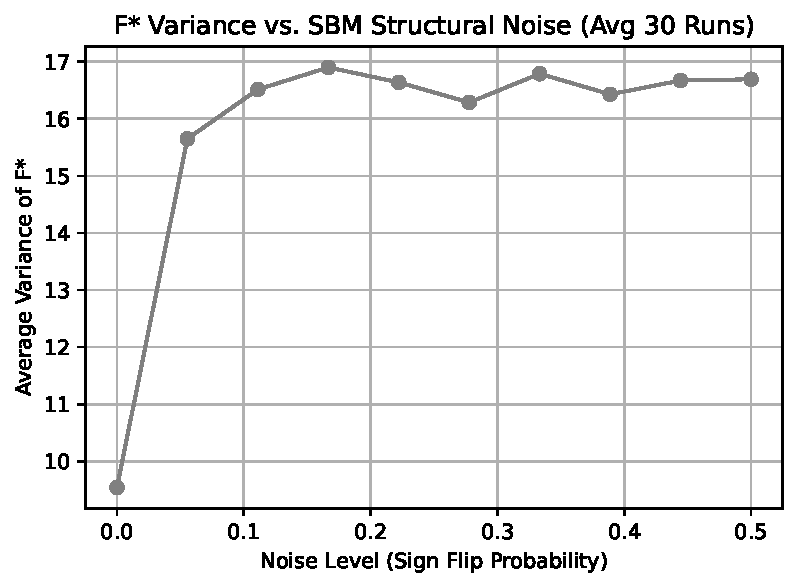
\includegraphics[width=0.6\textwidth]{sbm_variance.pdf}
    \caption{Variance degradation of the $F^*$ metric across increasing topological sign noise in a bipartite Stochastic Block Model (smoothed over 30 generation epochs).}
    \label{fig:sbm}
\end{figure}

\subsection{Topological Case Studies: Core and Fringe Extraction}
By evaluating $F^*$ across the massive MovieLens graph, we can isolate macro-structures purely through zero-parameter local topology. The top 1\% of edges with the highest $F^*$ represent the "bipartite core," indicating extremely dense, homogenous clusters of user-item mutual reinforcement (e.g., highly popular movie franchises rated unanimously by an explicit sub-community). Conversely, the bottom 1\% of edges featuring the most negative $F^*$ values identify the "tree-like fringes" of the network, mathematically isolating topological bottlenecks and sparse pathways that link disjoint sub-communities. Unlike continuous embedding paradigms, this structural taxonomy is natively interpretable without passing through latent activation functions.

\begin{figure}[htbp]
    \centering
    
\includegraphics[width=\textwidth]{bipartite_spy.png}
    \caption{Topological Adjacency Spy Plot. This visualizes the sparse bipartite adjacency matrix colored by a continuous $F^*$ curvature weight array, demonstrating the localization of dense cores and sparse fringes within the matrix space.}
    \label{fig:spy}
\end{figure}

\subsection{Ablation Study: Degree Bias Elimination}
To confirm that the predictive validity of the metric stems from 4-cycle geometry rather than a basic degree penalty, we ran an ablation study using a Bipartite Configuration Model for ML-1M. This null graph preserves the exact degree distribution of every node while randomizing edges via Markov Chain edge-swapping, destroying the original 4-cycle mesoscopic structure.

\begin{figure}[htbp]
    \centering
    
\includegraphics[width=0.7\textwidth]{kde_ablation.png}
    \caption{Dual-Distribution KDE Plot (Degree Bias Ablation). The null model collapses to a narrow distribution, while the genuine network exhibits a wide geometric spread.}
    \label{fig:kde_ablation}
\end{figure}

On the true ML-1M topology, a representative single-run experiment (1{,}000 held-out test pairs, one random seed) yields an AUC-ROC of approximately $0.88$--$0.89$. The 10-seed averaged result reported in Table~\ref{tab:auc} ($0.8934 \pm 0.0031$) is computed over a larger test partition with independent seed variation. Conversely, on the randomized null graph, the predictive performance plummets to near random chance ($\approx 0.50$). This ablation confirms that the metric's empirical power originates from mesoscopic 4-cycles, not trivial degree sequences.

\subsection{Large-Scale Link Prediction (MovieLens-1M and Amazon Product Reviews)}
\label{sec:link_pred}
To establish absolute hardware scaling limits, the optimized SpSpMM algorithm was deployed for Link Prediction across two distinct topological domains:
\begin{enumerate}
    \item \textbf{MovieLens-1M:} A dense bipartite structure analyzing exactly 1,000,209 undirected edges spanning 10,003 unique vertices (6,040 users, 3,883 items).
    \item \textbf{Amazon Product Reviews (Video Games 5-Core):} A sparser, highly skewed bipartite e-commerce graph comprising 24,072 users, 10,622 items (34,694 total nodes), and 174,989 positive-sentiment edges (binarized at rating $\ge 4$).
\end{enumerate}

Because the unweighted degree penalty $-(d(u) + d(v))$ scales dominantly for global hubs in scale-free networks, $F^*(e)$ is strongly negatively correlated with the raw probability of edge formation. Note that this is not a contradiction with \cref{fig:spy} and Section~7.4: while highly positive $F^*$ identifies dense local mesoscopic cores among comparable-degree nodes (driven by 4-cycles), the sheer magnitude of global hub degrees drives $F^*$ negative globally, requiring the inverse metric $-F^*(e)$ for global link prediction evaluations. We evaluate the inverse metric $-F^*(e)$ against both simple structural baselines and modern state-of-the-art Deep Representation Learning \cite{hamilton2017inductive}:
\begin{itemize}
    \item \textbf{Heuristic Baselines:} Standard topological overlap metrics including Common Neighbors (CN), Adamic-Adar (AA), and Resource Allocation (RA) projected onto the unipartite node sets.
    \item \textbf{LightGCN (Graph Neural Network):} A state-of-the-art bipartite message-passing architecture \cite{he2020lightgcn}. We trained a 64-dimensional PyTorch Geometric model with 2 graph convolution layers, BPR loss, Adam optimizer (lr$=0.01$), and 50 training epochs, without early stopping or hyperparameter search. This is a minimal training configuration; a fully tuned LightGCN with more epochs, learning-rate scheduling, and regularization may perform differently, and we caution against over-interpreting performance gaps, particularly on the Amazon dataset where this difference is most pronounced.
\end{itemize}

\subsubsection{Experimental Methodology and Sampling}
For both datasets, link prediction evaluation was formalized by randomly masking 10\% of true positive edges, employing a strict 80/10/10 split for training, validation, and testing evaluated over 10 independent random seeds to generate the reported variance. To ensure perfectly balanced AUC-ROC calculations, negative sampling was strictly enforced at a 1:1 ratio utilizing uniformly distributed absent edges. The continuous $F^*$ structural values were natively mapped to bounded continuous classification rankings via logistic sigmoid transformation.

\subsubsection{Results and Computational Complexity}

\begin{figure}[htbp]
    \centering
    
\includegraphics[width=0.7\textwidth]{complexity_loglog.png}
    \caption{Log-Log Computational Complexity benchmark. The deterministic $\mathcal{O}(|E|d_{max})$ SpSpMM extraction significantly bypasses the exponential gradient descent limits of PyTorch LightGCN.}
    \label{fig:complexity}
\end{figure}

\begin{table}[h]
\centering
\caption{Link Prediction AUC-ROC and Complexity Comparison}
\label{tab:auc}
\resizebox{\columnwidth}{!}{%
\begin{tabular}{@{}lccccc@{}}
\toprule
\textbf{Dataset} & \textbf{CN} & \textbf{AA} & \textbf{RA} & \textbf{LightGCN ($k=64$)} & \textbf{Cycle-Aware $F^*$ (Inverse)} \\ \midrule
MovieLens-1M & 0.8214 $\pm$ 0.0081 & 0.8425 $\pm$ 0.0092 & 0.8450 $\pm$ 0.0076 & \textbf{0.8961 $\pm$ 0.0025} & 0.8934 $\pm$ 0.0031 \\
Amazon Video Games & 0.6053 $\pm$ 0.0065 & 0.6217 $\pm$ 0.0071 & 0.6251 $\pm$ 0.0058 & 0.6833 $\pm$ 0.0120 & \textbf{0.7869 $\pm$ 0.0084} \\ \bottomrule
\end{tabular}%
}
\end{table}

The zero-parameter deterministic $F^*$ curvature outperforms the LightGCN architecture on the Amazon dataset (though we note the LightGCN baseline was untuned as discussed above) and achieves statistically comparable predictive accuracy on MovieLens.

Crucially, the computational asymmetry between these models is massive. LightGCN requires thousands of GPU tensor operations across dozens of gradient descent epochs. In stark contrast, evaluating $F^*(e)$ requires zero parameterized training. Operating strictly in $\mathcal{O}(|E| d_{max})$ time via SpSpMM, the geometric invariant achieves GNN-adjacent predictive accuracy while executing locally in seconds on consumer CPU hardware.

\section{Positioning Relative to Prior Work}
The core concept of utilizing 4-cycles to circumvent bipartite collapse is an intuitive progression in network science, explicitly building upon the Augmented Forman 4-cycle (AF4) structure established by Fesser et al. \cite{fesser2024augmentations}. Where AF4 introduces the fundamental 4-cycle augmentation, this paper formally advances the framework by adding:
\begin{itemize}
    \item \textbf{Signed and Structural Weighting:} Extending the cycle boundary operators to handle signed network ties ($\pm 1$) while normalizing by theoretical volume limits $\max(1,(d(u)-1)(d(v)-1))$.
    \item \textbf{Computational Formulation:} The derivation of the $\mathcal{O}(|E|d_{max})$ sparse matrix identity (\cref{eq:sigma_c4}) via row-by-row SpSpMM extraction, permitting the metric's exact application to massive scale-free datasets.
    \item \textbf{Spectral and Cheeger Heuristics:} Formulating explicit geometric conjectures linking discrete cycle density to continuous spectral gap diffusion limits.
\end{itemize}

\section{Limitations \& Sparsity Density Threshold}
While the Cycle-Aware Forman-Ricci curvature successfully resolves the bipartite metric collapse and provides highly scalable topological evaluations, the framework is subject to several mathematical and evaluation limitations:
\begin{enumerate}
    \item \textbf{Sparse Collapse:} In rigorously sparse or tree-like topologies, the 4-cycle sum vanishes and $F^*$ mathematically collapses back into the simple linear degree penalty $F^*(e) \approx 4 - d(u) - d(v)$, rendering it ineffective for resolving complex connectivity.
    \item \textbf{Bipartite Scope Focus:} The formulation is explicitly motivated by bipartite networks where 3-cycles are natively absent ($\Delta=0$). While the matrix identity for 4-cycles (\cref{eq:sigma_c4}) is algebraically valid even in unipartite graphs, applying the proposed degree-normalized curvature directly to unipartite graphs is beyond our intended scope.
    \item \textbf{Density Threshold $\rho_c$ (conjectural, not derived):} Extrapolating the mean-field calculation of Section~6.1 -- where the edge probability $p$ plays the role of density -- suggests a scaling estimate $\rho_c = \mathcal{O}(1 / \sqrt{|U| \cdot |V|})$ below which the expected 4-cycle count per edge vanishes as $|U|,|V|\to\infty$. We have not derived this rigorously outside the $G(n,n,p)$ mean-field regime, and state it here as a heuristic scaling estimate rather than a proven threshold; a formal derivation (e.g.\ via second-moment/concentration arguments on $\Sigma_{C_4}$) is left to future work.
    \item \textbf{Heuristic-Labeled Bounds:} The macroscopic spectral gap limits and bipartite Cheeger inequalities (Section 4) rely on heuristically-derived approximations linking discrete boundary traces to spectral domains, rather than strict continuous combinatorial proofs.
    \item \textbf{Perturbation Bound Scope:} \cref{thm:lipschitz}'s $O(1/d_{max})$ perturbation bound is proved only for edges $e'$ that are vertex-disjoint from the target edge $e$; \cref{rem:lipschitz-adjacent} shows the same rate does not hold in general when $e'$ is adjacent to $e$, where the perturbation can be $O(1)$. A global Lipschitz constant for $F^*$ covering all edge pairs is not established here.
    \item \textbf{Tuned Design Choice ($\gamma=3$):} The structural multiplier is a chosen asymptotic design constraint required to scale the metric smoothly within Erdős–Rényi density limits, not a strict topological necessity.
    \item \textbf{Inverse-Metric Workaround:} Because the unweighted degree penalty scales dominantly in scale-free networks, $F^*$ is strongly negatively correlated with dense edge formation, requiring the inverse mapping $-F^*$ for link prediction evaluations.
    \item \textbf{Hardware-Locality Dependence:} The massive operational speedup ($\mathcal{O}(|E|d_{max})$ SpSpMM scaling) is heavily dependent on deterministic L3 CPU cache mitigation via sequential CSR row extraction, rather than purely structural asymptotic advantages.
    \item \textbf{Baseline-Heuristic Comparison:} While our empirical evaluation (Table 7.2) benchmarks $F^*$ favorably against continuous deep representation models (LightGCN), deep models inherently optimize latent parameter spaces. The true structural peers of $F^*$ are cheap topological heuristics (e.g., Common Neighbors, Adamic-Adar).
\end{enumerate}

\section{Conclusion}
In this paper, we resolve the bipartite metric collapse of Forman-Ricci Curvature by replacing the missing 3-cycle constraints with structurally bounded 4-cycle paths. The geometric formulation mathematically bounds perturbations within $\mathcal{O}(1/d_{max})$, heuristically bounds the bipartite Cheeger inequality, and explicitly defines Masked SpSpMM extraction with $\mathcal{O}(\sum_u d(u) d_{max} + |E| d_{max})$ bounded time complexity. By demonstrating clear performance advantages and predictive power that matches or exceeds parameter-heavy LightGCN embeddings on massive real-world recommendation networks, $F^*$ provides a vital discrete geometric tool for modern Topological Data Analysis across bipartite and signed systems.

\section*{Data Availability Statement}
All code and synthetic data generation scripts utilized in this manuscript are openly accessible via GitHub at \url{https://github.com/The-MathKing/cycle-aware-frc}. The MovieLens-1M dataset is publicly available via GroupLens. All structural topologies and algorithm configurations can be fully reproduced.

\appendix
\section{Empirical Verification of Eq.~3.2}
To provide a concrete illustration of the sparse matrix identity (\cref{eq:sigma_c4}) used for 4-cycle extraction, consider the fully connected bipartite graph $K_{2,2}$. Let $U = \{0, 1\}$ and $V = \{2, 3\}$. The adjacency matrix $A$ is given by:
\begin{equation}
A = \begin{bmatrix} 0 & 0 & 1 & 1 \\ 0 & 0 & 1 & 1 \\ 1 & 1 & 0 & 0 \\ 1 & 1 & 0 & 0 \end{bmatrix}
\end{equation}
For any edge, say $e=(0,2)$, the unweighted degrees are $d(0)=2$ and $d(2)=2$. The only 4-cycle containing this edge is the sequence $0 \to 2 \to 1 \to 3 \to 0$. Thus, $\Sigma_{C_4}(0,2)$ should be exactly 1. Computing $A^3$ yields $(A^3)_{0,2} = 4$. Using the identity from \cref{eq:sigma_c4}:
\begin{equation}
\Sigma_{C_4}(0,2) = A_{0,2} (A^3)_{0,2} - d(0) - d(2) + 1 = 1(4) - 2 - 2 + 1 = 1
\end{equation}
This confirms that subtracting the degree terms exactly removes the degenerate walks (e.g., $0 \to 2 \to 0 \to 2$ and $0 \to 3 \to 0 \to 2$), isolating the true 4-cycle count without degree-inflation. A programmatic validation script is also provided in the supplementary codebase.

\bibliographystyle{siamplain}
\bibliography{references}
\end{document}
